\paragraph[QuizziPedia::Front-End::ModelViews\\::CreateQuestionnaireModelView]{QuizziPedia::Front-End::ModelViews::CreateQuestionnaireModelView}
	
	\label{QuizziPedia::Front-End::ModelViews::CreateQuestionnaireModelView}
	
	\begin{figure}[ht]
		\centering
		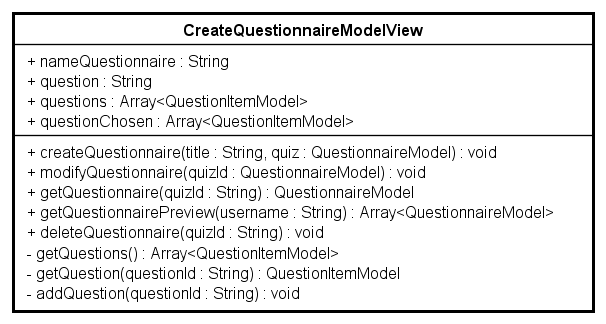
\includegraphics[scale=0.5,keepaspectratio]{UML/Classi/Front-End/QuizziPedia_Front-end_ModelView_CreateQuestionnaireModelView.png}
		\caption{QuizziPedia::Front-End::ModelViews::CreateQuestionnaireModelView}
	\end{figure} \FloatBarrier
	
	\begin{itemize}
		\item \textbf{Descrizione}: classe di tipo modelview la cui istanziazione è contenuta all'interno della variabile di ambiente \texttt{\$scope} di \textit{Angular\ped{G}}. All'interno di essa sono presenti le variabili e i metodi necessari per il \textit{Two-Way Data-Binding\ped{G}} tra la \textit{view\ped{G}} \texttt{CreateQuestionnaireView} e il \textit{controller\ped{G}} \texttt{CreateQuestionnaireController};
		\item \textbf{Utilizzo}: viene utilizzata per effettuare il \textit{Two-Way Data-Binding\ped{G}} tra la \textit{view\ped{G}}\\ \texttt{CreateQuestionnaireView} e il \textit{controller\ped{G}} \texttt{CreateQuestionnaireController} rendendo disponibili variabili e metodi;
		\item \textbf{Relazioni con altre classi}: 
		\begin{itemize}
			\item \textbf{OUT \texttt{CreateQuestionnaireView}}: \textit{view\ped{G}} per la creazione del questionario; 
			\item \textbf{OUT \texttt{CreateQuestionnaireController}}: questa classe permette di gestire la creazione di un questionario.
		\end{itemize}
		\item \textbf{Attributi}: 
		\begin{itemize}
			\item \texttt{+ nameQuestionnaire: String}: \\ Attributo che specifica il nome del questionario creato;
			\item \texttt{+ question: String} \\ Attributo che conterrà la stringa per la ricerca della domanda;
			\item \texttt{+ questions: Array<QuestionItemModel>} \\ \texttt{array} contenente le domande trovate durante la ricerca;
			\item \texttt{+ questionsChosen: Array<QuestionItemModel>} \\ \texttt{array} contenente le domande inserite nel questionario.
		\end{itemize}
		\item \textbf{Metodi}: 
		\begin{itemize}
			\item \texttt{+ createQuestionnaire(title: String, \\quiz: QuestionnaireModel) : void} \\Metodo che permette di inserire un questionario nel database tramite richiesta al service. \\
			\textbf{Parametri}:
			\begin{itemize}
				\item \texttt{title: String} \\ Parametro che indica il nome del questionario;
				\item \texttt{quiz: QuestionnaireModel} \\ Parametro che racchiude tutti i dati di un questionario.
			\end{itemize}
			\item \texttt{+ modifyQuestionnaire(quizId: QuestionnaireModel): void} \\ Metodo che serve per modificare un questionario. \\
			\textbf{Parametri}:
			\begin{itemize}
				\item \texttt{quiz: QuestionnaireModel}\\
				Parametro che rappresenta l'oggetto questionario.
			\end{itemize}
			\item \texttt{+ getQuestionnaire(quizId: String): QuestionnaireModel} \\Metodo che serve per ottenere un questionario tramite l'id in modo da poterlo modificare. \\
			\textbf{Parametri}:
			\begin{itemize}
				\item \texttt{quizId: String}\\
				Parametro che rappresenta l'id del questionario da richiedere.
			\end{itemize}
			\item \texttt{+ getQuestionnairePreview(username: String): Array<QuestionnaireModel>} \\ Metodo che serve per ottenere la lista di tutti i questionari di un utente. \\
			\textbf{Parametri}:
			\begin{itemize}
				\item \texttt{username: String}\\
				Parametro che indica l'utente del quale vogliamo caricare tutti i questionari.
			\end{itemize}
			\item \texttt{+ deleteQuestionnaire(quizId: String): void} \\ 
			Metodo che elimina un questionario. \\
			\textbf{Parametri}:
			\begin{itemize}
				\item \texttt{quizId: String}\\
				Identificativo del questionario da eliminare.
			\end{itemize}
			
			\item \texttt{+ getQuestions(): Array<QuestionItemModel>} \\
			Metodo che permette di ottenere la lista di tutte le domande.
			
			\item \texttt{+ getQuestion(questionId: String): QuestionItemModel} \\
			Metodo che ritorna l'intera domanda selezionata. \\
			\textbf{Parametri}:
			\begin{itemize}
				\item \texttt{questionId: String}\\
				Parametro che indica l'identificativo univoco di una domanda.
			\end{itemize}
			\item \texttt{+ addQuestion(questionId: String) : void} \\
			Metodo che permette di inserire una domanda nel questionario. \\
			\textbf{Parametri}:
			\begin{itemize}
				\item \texttt{questionId: String}\\
				Parametro che indica l'identificativo univoco di una domanda.
			\end{itemize}
			\item \texttt{+} \texttt{showAllQuestions(topic: String, keyword: String): void} \\
			Metodo che permette di ottenere la lista di tutte le domande ed inserirle nello \$scope nell'oggetto di tipo \texttt{CreateQuestionnaireModelView}.\\
			\textbf{Parametri}:
			\begin{itemize}
				\item \texttt{topic: String}\\ Parametro che indica l'argomento scelto;
				\item \texttt{keyword: String}\\ Parametro che indica la parola chiave scelta.
			\end{itemize}
			\item \texttt{+} \texttt{createQMLQuestion(question: String) : void} \\
			Metodo che permette di posizionarsi nella pagina dell'editor QML;\\
			\item \texttt{+} \texttt{filterByYours(question: String) : QuestionItemModelView} \\
			Metodo che permette di rimuovere una domanda nel questionario.\\
			\textbf{Parametri}:
			\begin{itemize}
				\item \texttt{question: String}\\ Parametro che la domanda da filtrare.
			\end{itemize}
			\item \texttt{+} \texttt{resetFilters() : void} \\
			Metodo che permette di resettare i filtri finora settati;\\
			\item \texttt{+} \texttt{noFilter(filterObj: Array<Boolean>) : QuestionItemModelView} \\
			Metodo che permette di filtrare un array.\\
			\textbf{Parametri}:
			\begin{itemize}
				\item \texttt{filterObj: Array<Boolean>}\\ Parametro contenente un array di boolean.
			\end{itemize}
		\end{itemize}
	\end{itemize}
	
	